\documentclass[10pt,a4paper]{article}
\usepackage[utf8]{inputenc}
\usepackage{amsmath}
\usepackage{amsfonts}
\usepackage{amssymb}
\usepackage{graphicx}
\usepackage[left=30mm, right=20mm, top=30mm, bottom=30mm]{geometry}
\usepackage[german]{babel}
\usepackage{graphicx,array}
\usepackage{fancyhdr}
\usepackage{setspace}
\usepackage{wrapfig}

\begin{document}
	\author{Peter Pollheimer, Jakob Tomasi, Elias Gabl}
	\date{\today}
	\title{Systemdokumentation}
	
	\lfoot{IT Kolleg Imst | 4AAIF}
	\cfoot{Jakob Tomasi, Peter Pollheimer, Elias Gabl}
	\rfoot{Seite \thepage}
	
	\lhead{Communicational}
	\chead{}
	\rhead{Systemdokumentation}
	
	\maketitle
	
	\begin{figure}[h]
		\centering
		
\includegraphics[scale=0.6]{pictures/itkolleg_logo.pdf}
	\end{figure}
	
	\thispagestyle{empty}
	\newpage
	\thispagestyle{empty}
	\tableofcontents
	\newpage
	\pagestyle{fancy}
	\doublespacing
	
	\section{Verwendete Technologie}
	\subsection{OSTicket}
	OSTicket ist ein weit verbreitetes, quelloffenes Ticketingsystem. Es verfügt über eine zentrale MySQL-Datenbank und ein Multi-User Web Interface. Dieses Webinterface gilt es im Zuge dieses Projektes so aufzubereiten, dass es neben den üblichen Auflösungen von Desktop- und Laptopbildschirmen auch Mobile Displays wie die von Smartphones oder Tablets unterstützt.
	
	\begin{wrapfigure}{r}{0.4\textwidth}
		\vspace{-1cm}
		\begin{center}
		\caption{OSTicket Logo}
		\vspace{.5cm}
		
\includegraphics[scale=.7]{pictures/icon_osticket.png}
		
		\label{OSTicket Logo}
		\end{center}
	\end{wrapfigure}

	Es wird eine Minimum-Impact Strategie verfolgt, das heißt dass im Zuge der Projektdurchführung die Änderungen auf das Vanilla-System so gering als möglich ausfallen. Damit wird einerseits das Ziel verfolgt, eine gewisse Übersichtlichkeit zu bewahren, was in einer kompakten Dokumentation resultieren soll.
	
	Des weiteren sollen nicht benötigte Funktionalitäten bewahrt bleiben, um systeminterne Reibungen zu vermeiden und Funktionen im Nachhinein mit geringem Aufwand verwenden zu können.
	
	\begin{figure}[h]
		\centering
		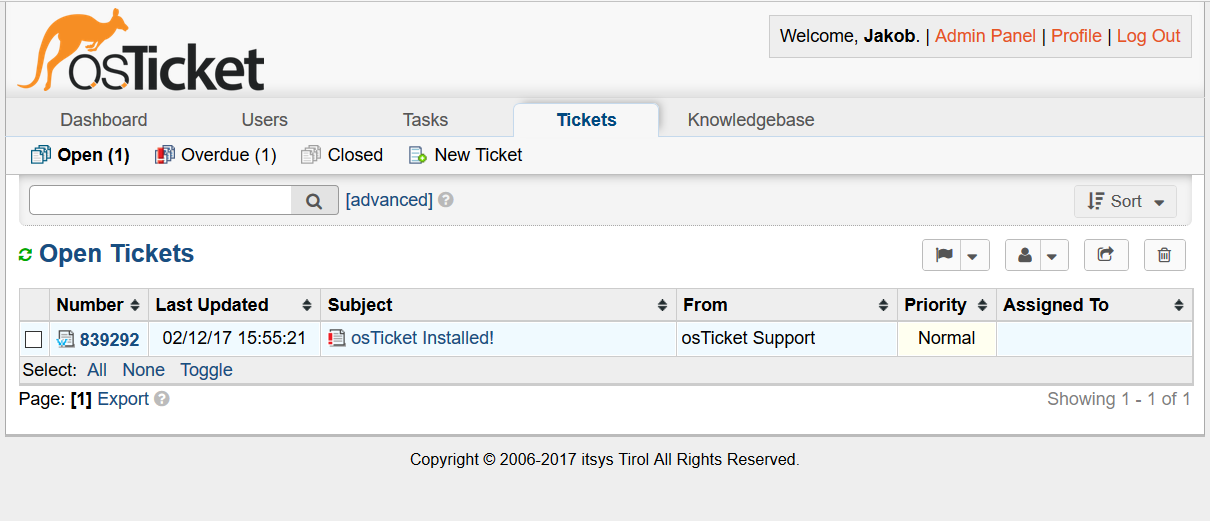
\includegraphics[scale=0.62]{pictures/osticket.png}
		\caption{Die standard-Weboberfläche für Administratoren}
		\label{OSTicket Admin WebGUI}
	\end{figure}

	\subsubsection{M"oglichkeiten mit OSTicket}
	OSTicket ist sehr anpassbar. Ticketformulare und Formularfelder lassen sich mit geringem Aufwand anpassen, je nach den spezifischen Anforderungen des Helpdesks. Sollte einmal ein wahrer Sturm an Tickets eingehen, ist auch das kein Problem. Tickets lassen sich simpel priorisieren und filtern. Noch mehr Übersicht bringt die M"oglichkeit, Tickets in Hilfsthematiken einzustufen. Sollten mehrere Supportmitarbeiter gleichzeitig Arbeiten, geschieht dies ohne Problem: Ticketkollisionen werden automatisch mit Sperrvariablen vermieden.
	
	\subsubsection{Warum OSTicket?}
	Es gibt viele Gründe die für die Verwendung der Plattform OSTicket sprechen. OSTicket findet bereits bei einigen Schulen in Tirol Anwendung. Dies soll beibehalten und auf weitere Schulen ausgeweitet werden.
	\\
	Die Vorteile dieser Verbreitung und der damit einher gehenden Standardisierung kann für die Schulen große Vorteile mit sich bringen. Die bis jetzt verwendeten Systeme sind sehr unterschiedlich und in keiner Weise miteinander kompatibel. OSTicket soll als anwenderfreundliches System diese Schwierigkeiten vermeiden und beseitigen. Dadurch soll eine bessere Kommunikation zwischen Systembetreuern und IT Managern an Tirols Schulen ermöglicht werden.

	\subsection{Bootstrap}
	Das Framework Bootstrap wird verwendet, um eine Anwender freundliche Mobile-first Oberfläche zu erstellen. Bootstrap bietet umfangreiche Gestaltungsvorlagen wie Formulare, Buttons, Tabellen und weitere nützliche Oberflächengestaltungssysteme.
	
	\begin{figure}[h]
		\centering
		
\includegraphics[scale=0.65]{pictures/twitter-bootstrap.jpg}
		\caption{Twitter Bootstrap Logo}
		\label{Bootstrap_Logo}
	\end{figure}
	
	Gründe die für die Verwendung von Bootstrap sprechen:
	\begin{itemize}
		\item Responsive-Design
		\item Hohe Kompatibilität bezüglich Browser
		\item Übersichtliche Dokumentation 
		\item Eine Vielzahl von Templates ist verfügbar
	\end{itemize}
\begin{figure}[h]
	\centering
	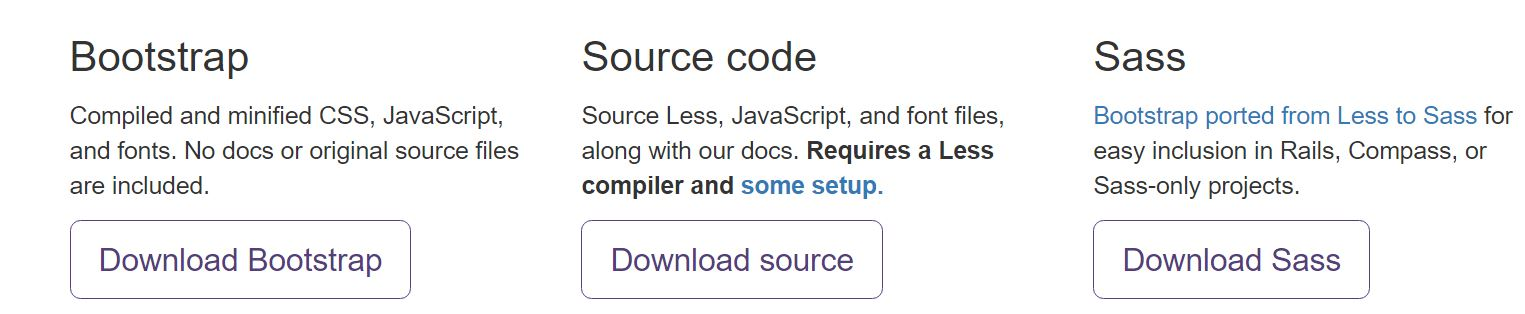
\includegraphics[scale=0.7]{pictures/bootstrap.jpg}
	\caption{Bootstrap ist ein vielseitiges und anpassbares Framework}
	\label{Bootstrap Page Screenshot}
\end{figure}
	\subsection{PHP}
	OSTicket basiert auf der Skriptsprache PHP. PHP ist ein rekursives Akronym und bedeutet "Hypertext Preprocessor". PHP kann direkt in HTML\footnote{Hypertext Markup Language, definiert das Grundgerüst einer Webseite} eingebettet werden. Die Skriptsprache bietet eine Vielzahl an Funktionen Out Of The Box, wie zum Beispiel das Senden und Empfangen von Emails, Manipulation einer Datenbank oder das Befüllen einer Webseite mit Inhalten.
	
	\begin{figure}[h]
		\centering
		
\includegraphics[scale=.6]{pictures/php_logo.png}
		\caption{PHP Ver. 7 Logo}
		\label{PHP_Logo}
	\end{figure}
	
	PHP ist der etablierte Standard, wenn es um serverseitige Webprogrammierung geht. Serverseitige Webprogrammierung findet statt, wenn ein Benutzer mit seinem Browser\footnote{Software zum Benutzen des World Wide Web; Bspw. Microsoft Internet Explorer, Mozilla Firefox} eine Webseite ansurft. Es wird eine sogenannte HTTP-Anfrage an den Webserver (welcher unter der Webseitenadresse erreichbar ist) gesendet. Dieser analysiert die Anfrage (welche Seite der Benutzer sehen will) und befüllt das HTML-Grundgerüst mit dynamischen Inhalten. Dann wird die Seite über das Internet zurück zum Browser des Benutzers übertragen und dargestellt.
	
	Ein großer Vorteil von PHP ist, dass es für Einsteiger in die Programmierung gut zu erlernen ist, dennoch aber äußerst flexibel, um auch umfangreiche Anwendungen (Wie OSTicket) umsetzen zu können. \\
	Die Flexibilität von PHP zeigt sich auch in der Freiheit, es auf vielen unterschiedlichen Betriebssystem wie Microsoft Windows, Apple OSX und einer Vielzahl an Linuxdistributionen verwenden zu können. Auch allerhand Webserver verstehen PHP wie ihre Muttersprache: Apache, IIS und nginx, um nur einige zu nennen.
	
	\subsection{MySQL}
	MySQL ist ein Datenbanksystem das weltweit verbreitet ist. Es gibt eine Open-Source-Sofware aber auch eine kommerzielle Enterpriseversion.
	
	\begin{figure}[h]
		\centering
		
\includegraphics[scale=.35]{pictures/mysql_logo.png}
		\caption{MySQL Logo}
		\label{MySQL_Logo}
	\end{figure}
	
	MySQL wird für die Datenspeicherung von Webservices verwendet. Es wird meistens zusammen mit dem Apache Webserver und der Skiptsprache PHP verwendet. Dies war auch der Grund weshalb wir MySQL verwenden da OSTicket in der Skriptsprache PHP geschrieben ist.
	MySQL und die Bibliotheken sind hauptsächlich in C und C++ geschrieben. Dies ist zurückzuführen auf die Erzielung einer gute Performance.
	MySQL sieht grundsätzlich eine MySQL-Server vor auf dem mehrere Datenbanken erstellt werden können. In einer Datenbank könne auch mehrere Tabellen erstellt werden.
	
	\newpage
	\section{Werkzeuge}
	Die im Zuge der Projektdurchführung verwendeten Werkzeuge eignen sich für das Projekt aus verschiedenen Gründen.
	
	Ein wichtiger Punkt war die Vertrautheit mit den Werkzeugen: Ein Großteil dieser war uns bereits bekannt beziehungsweise vertraut. Des Weiteren ist die große Community im Internet sehr hilfreich bei auftretenden Problemen und Fragestellungen; meist ist die Lösung innerhalb weniger Minuten gefunden. Da es sich um weit verbreitete Entwicklungsumgebungen handelt konnte auch in der Zukunft (während der Zeit der Projektdurchführung) mit der Weiterentwicklung und Verbesserung dieser Tools gerechnet werden.
	
	\subsection{NetBeans}
	Die integrierte Entwicklungsumgebung NetBeans ist in Java geschrieben und bietet vielerlei Funktionen wie einen umfangreichen Editor, eine passable Codevervollständigung, Code Analysetools, Debugger und kann mit hilfreichen Plug-Ins wie beispielsweise EasyUML, einem Programm zum Erstellen von UML-Klassendiagrammen aus einem vorhandenen Projekt, erweitert werden. Wie in der Abbildung \ref{Netbeans_GUI} zu sehen ist, kann das Farbthema der Entwicklungsumgebung angepasst werden. Das schont die Augen und erhöht den Workflow.
	
	\begin{figure}[h]
		\centering
		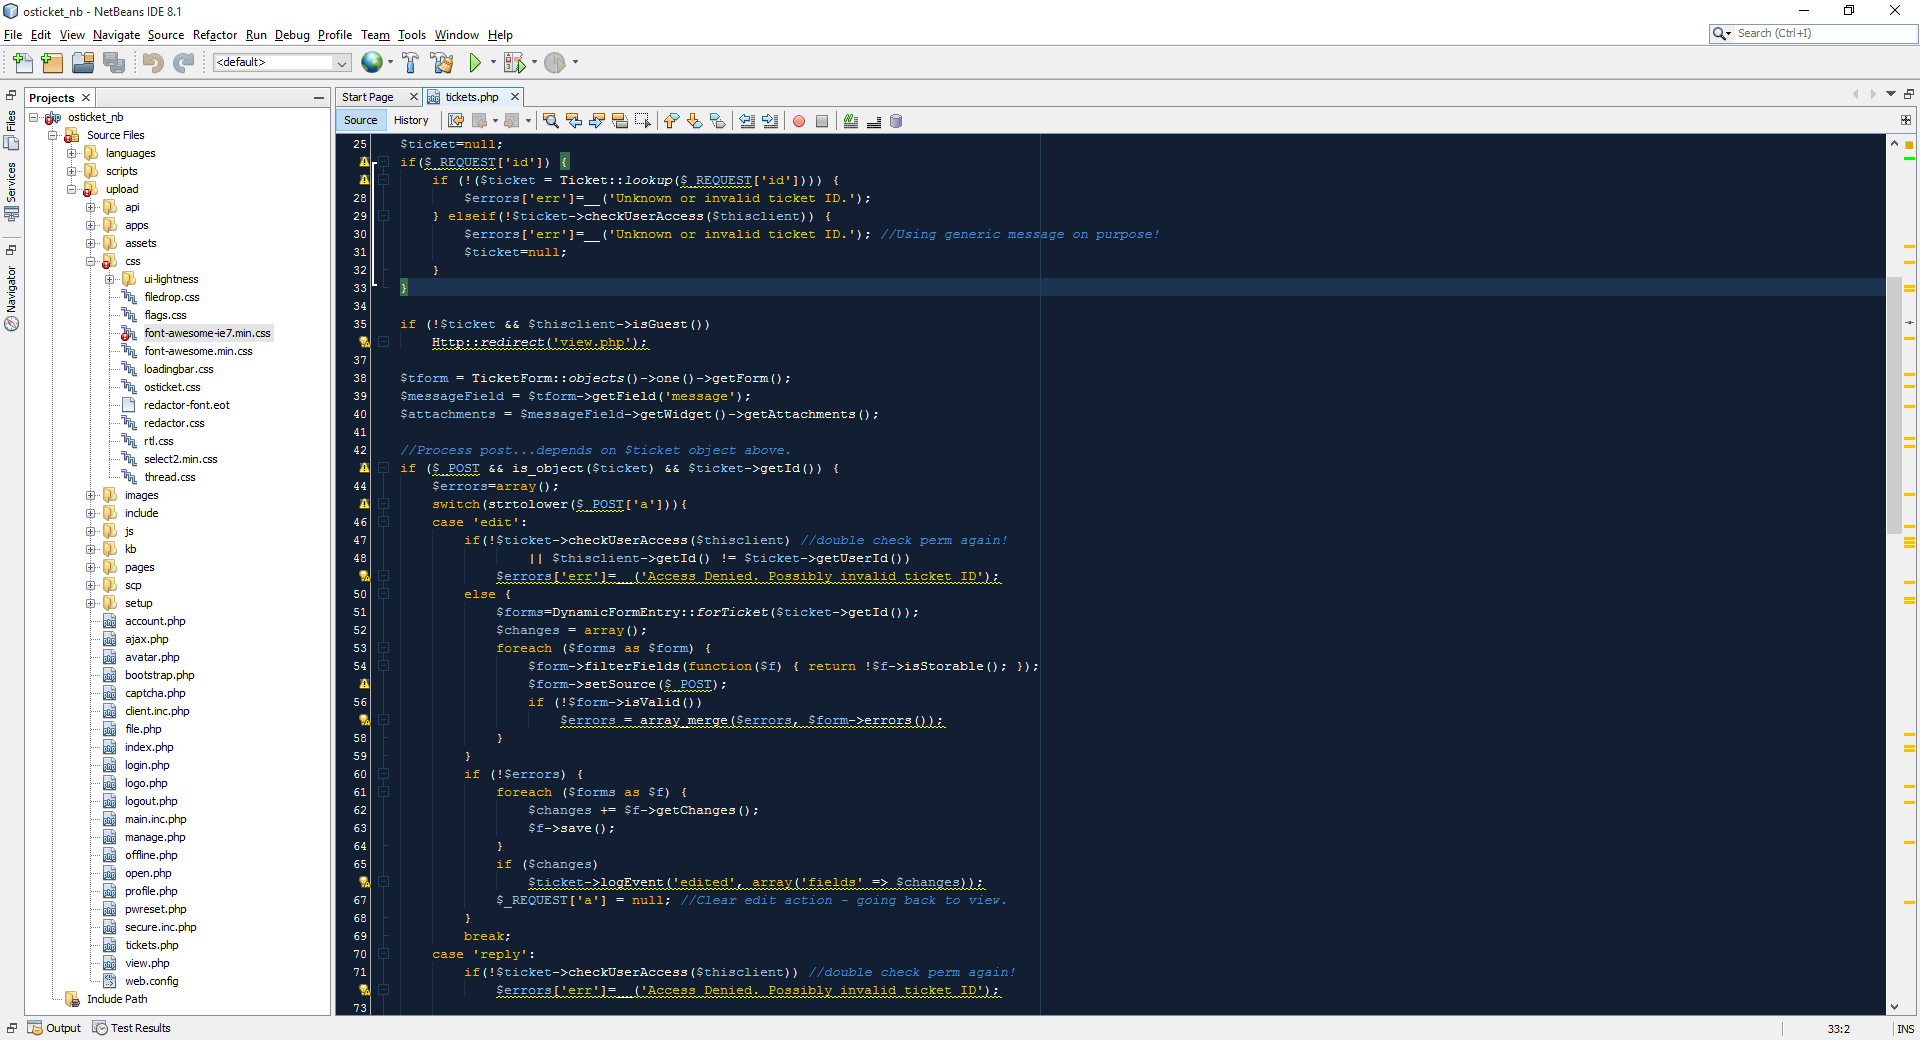
\includegraphics[scale=.3]{pictures/netbeans_gui.png}
		\caption{Netbeans User Interface}
		\label{Netbeans_GUI}
	\end{figure}
	
	\begin{wrapfigure}{r}{0.4\textwidth}
		\vspace{-1cm}
		\begin{center}
			\caption{Netbeans IDE Logo}
			\vspace{.5cm}
			
\includegraphics[scale=.39]{pictures/netbeans_logo.jpg}
			
			\label{Netbeans_Logo}
		\end{center}
	\end{wrapfigure}
	
	NetBeans unterstützt Programmiersprachen wie Java, PHP, C/C++ und andere. Des Weiteren ist NetBeans plattformunabhängig - wir als Projektteam haben somit die freie Wahl unter welchem Betriebssystem gearbeitet werden soll - die Kompatibilität unserer Ergebnisse ist jederzeit gegeben.
	\\
	Jedes neue Release wird auch von der Community getestet und evaluiert. Somit ist auch eine Hilfestellung bei Problemen gegeben.
	\subsection{XAMPP Apache}
	XAMPP ist eine Zusammenführung von freier Software. Es ermöglicht einfache Installation und Konfiguration des Webservers Apache und der Datenbank MariaDB. Weitere Anwendungen geliefert unter XAMPP sind die FTP-Server ProFTPd oder FileZilla Server, der Mailserver Mercury, der webbasierte Datenbankclient phpMyAdmin und andere offene Software.
	
	
	\begin{figure}[h]
		\centering
		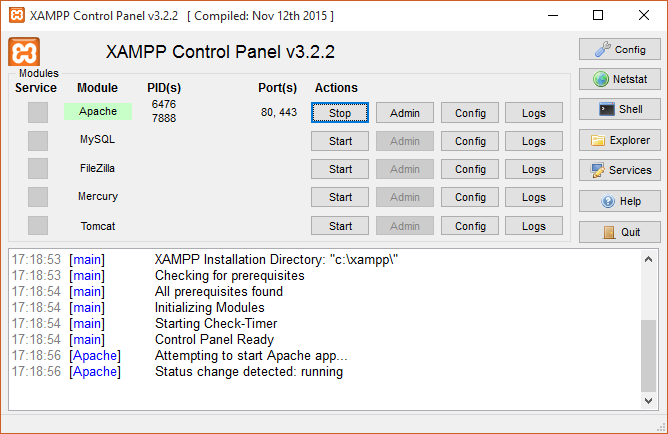
\includegraphics[scale=.8]{pictures/xampp_gui.png}
		\caption{XAMPP Control Panel}
		\label{XAMPP_GUI}
	\end{figure}

	\begin{wrapfigure}{r}{0.4\textwidth}
		\vspace{-1cm}
		\begin{center}
			\caption{XAMPP Logo}
			\vspace{.5cm}
			
\includegraphics[scale=.2]{pictures/xampp_logo.jpg}
			
			\label{XAMPP_Logo}
		\end{center}
	\end{wrapfigure}

	\newpage
	XAMPP ermöglicht eine einfache und schnelle Installation einer Testumgebung. Da XAMPP ausschließlich für Testumgebungen gedacht ist sind standardmäßige Sicherheitseinstellungen nicht ausreichend und ist somit nicht für Produktivumgebungen geeignet.
	
	
	\subsection{MySQL Workbench}
	Die Verwaltung der Verwendeten MySQL Datenbank erfolgt mit dem Tool MySQL Workbench. Die vielen Überwachungs- und Konfigurationsmöglichkeiten, die die GUI\footnote{Graphical User Interface} bietet, macht es möglich, auf aufwändige SQL-Skripte zu verzichten. Damit ist eine einfache Verwaltung und ein erleichterter Umgang mit dieser umfangreichen Datenbank gegeben.
	
	\begin{figure}[h]
		\centering
		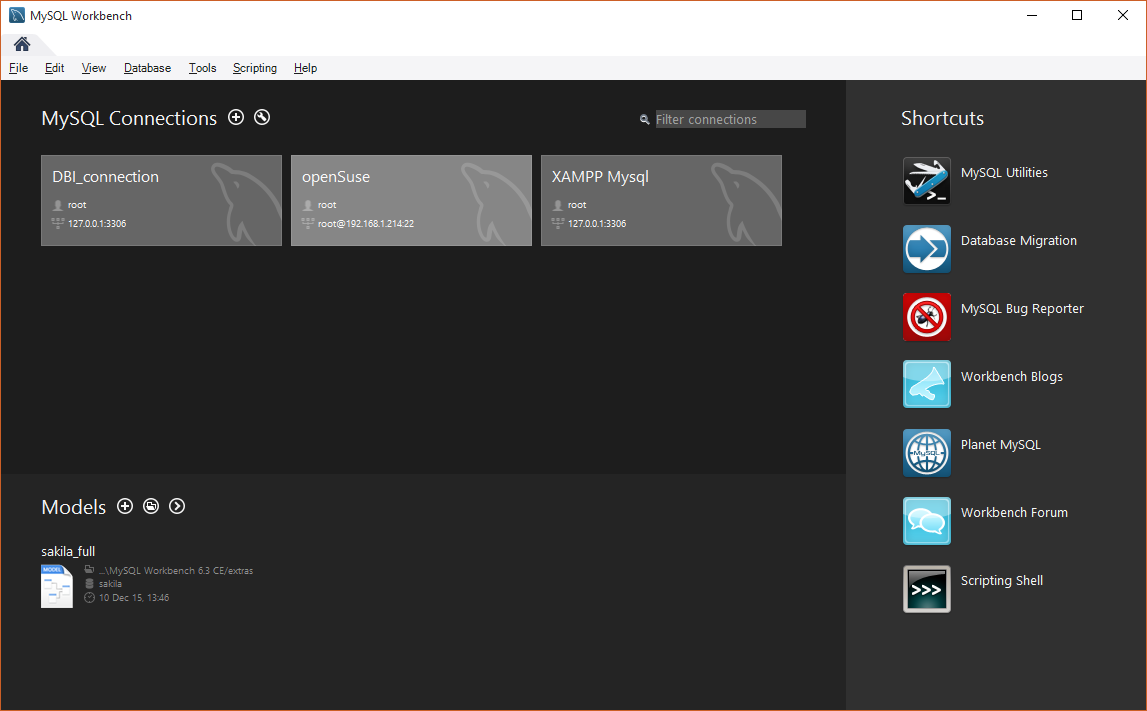
\includegraphics[scale=.5]{pictures/workbench_startgui.png}
		\caption{MySQL Workbench Start Screen}
		\label{Worbench_Startgui}
	\end{figure}

	Auch die Unterstützung von Projektbetreuern und weiteren Lehrpersonen kann in Betracht gezogen werden, da die MySQL Workbench im Unterricht oft Verwendung findet.
	
	\newpage

	\begin{figure}[h]
		\centering
		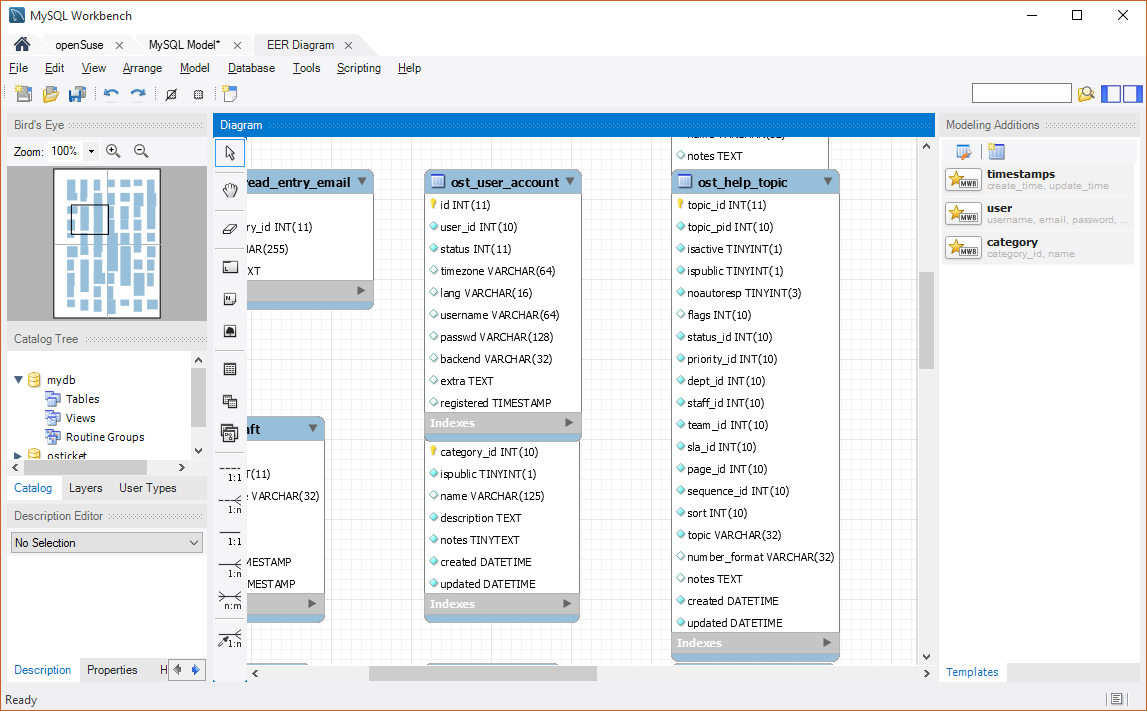
\includegraphics[scale=.5]{pictures/workbench_reverse.png}
		\caption{MySQL Workbench - Datenbankdiagramm (Ausschnitt)}
		\label{Workbench_DiaGUI}
	\end{figure}
		
	MySQL Workbench kann neben der Ausführung von Konfigurations- und Datenmanipulationsbefehlen auch Modellierung: Mit dem Integrierten UML Editor kann eine Datenbank (und die zugehörigen SQL Befehle) generiert werden. Auch die entgegengesetzte Richtung ist möglich: Mit wenigen Klicks kann ein UML Diagramm aus einer bestehenden Datenbank erstellt werden. Abbldung \ref{Workbench_DiaGUI} zeigt ein solches Klassendiagramm im Detail.
	
		
	\newpage
	\section{Modelle}
	\subsection{Klassendiagramm}
	Abbildung \ref{Klassendiagramm_System} soll die Klassen welche unter dem Ticketsystem Verwendung finden umreißend beschreiben. Das Diagramm dokumentiert nicht den kompletten systematischen Aufbau des Ticketsystems in seinem "Vanilla-Zustand"\footnote{"Vanilla" beschreibt ein System oder Produkt, welches in keinster Weise verändert (customized) worden ist.}, sondern ist eine Zusammenfassung der wichtigsten Klassen, die Anwendung finden und soll lediglich veranschaulichen, welche die fundamentalsten Klassen sind und in welchem Zusammenhang diese stehen.
	\begin{figure}[h]
		\centering
		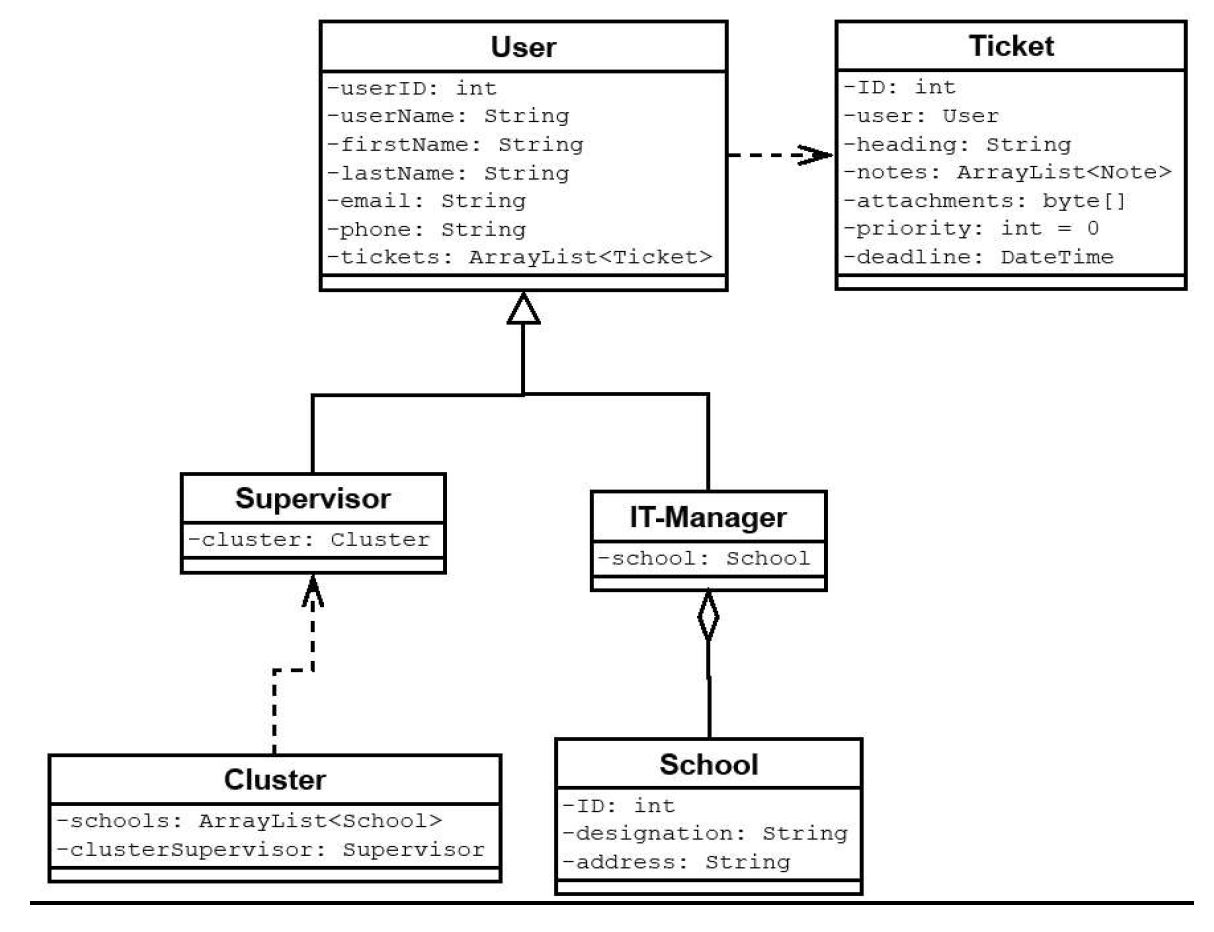
\includegraphics[scale=0.9]{pictures/Klassendiagramm.jpg}
		\caption{Komprimiertes Klassendiagramm}
		\label{Klassendiagramm_System}
	\end{figure}
	\newpage
	\subsection{Komponentendiagramm}
	\begin{figure}[h]
		\centering
		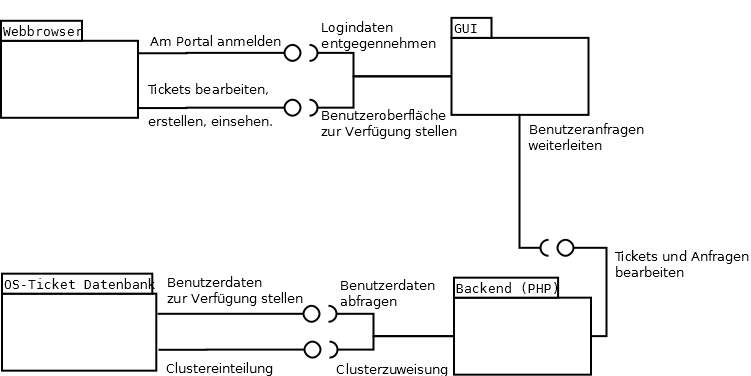
\includegraphics[scale=0.6]{pictures/Komponentendiagramm.png}
		\caption{Komponentendiagramm}
		\label{Komponentendiagramm}
	\end{figure}

	\newpage
	\section{Implementierung}
	Bis jetzt wurden wichtige GUI Elemente erstellt und bezüglich der Funktionalität mit unserem Projektpartner besprochen.
	\begin{figure}[h]
		\centering
		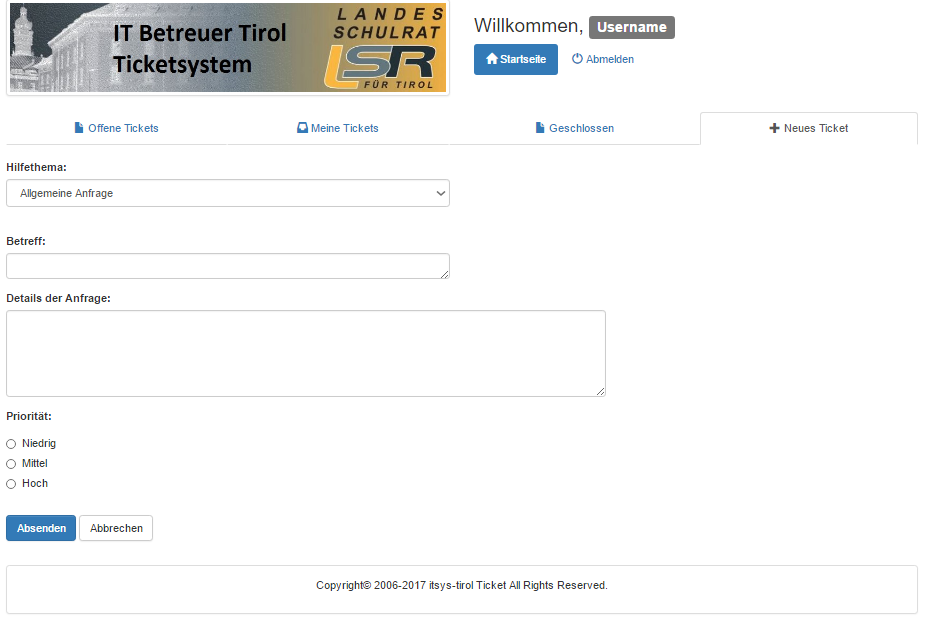
\includegraphics[scale=0.6]{pictures/newTicket.png}
		\caption{Ticket erstellen}
		\label{Ein Ticket erstellen}
	\end{figure}
	\begin{figure}[h]
		\centering
		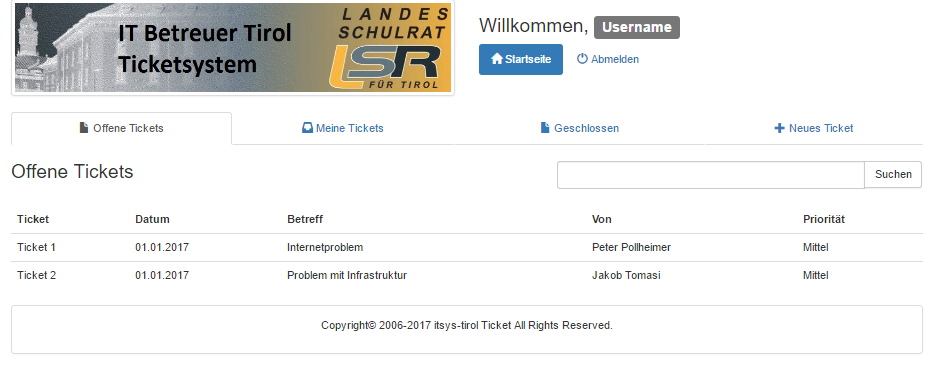
\includegraphics[scale=0.6]{pictures/index.png}
		\caption{Ticketverwaltung}
		\label{Tickets verwalten}
	\end{figure}
	
	
	
	
	
	\newpage
	\listoffigures
	
	\newpage
	\listoftables
\end{document}